\documentclass{beamer}

\usepackage[english,russian]{babel}
\usepackage{fontspec}
\usepackage{amsmath}
\usepackage{amssymb}
\usepackage{amsthm}
\usepackage{graphicx}

\makeatletter
\newenvironment{sqcases}{%
  \matrix@check\sqcases\env@sqcases
}{%
  \endarray\right.%
}
\def\env@sqcases{%
  \let\@ifnextchar\new@ifnextchar
  \left\lbrack
  \def\arraystretch{1.2}%
  \array{@{}l@{\quad}l@{}}%
}
\makeatother

\usefonttheme{serif}
\setmainfont{Liberation Serif}

\usetheme{Frankfurt}

\newtheorem{my_definition}{Определение}
\newtheorem{my_theorem}{Теорема}
\newtheorem{my_consequence}{Следствие}
\newtheorem{my_note}{Замечание}
\newtheorem{my_lemma}{Лемма}
\newtheorem{my_hypothesis}{Гипотеза}
\newtheorem{notation}{Обозначение}

\newcommand{\N}{\mathbb{N}}
\newcommand{\Z}{\mathbb{Z}}
\newcommand{\A}{\mathcal{A}}
\newcommand{\F}{\mathcal{F}}
\newcommand{\G}{\mathcal{G}}
\newcommand{\M}{\mathcal{M}}

\title{Вычисление функций автоматами со счётчиками}
\author{Илхомов Мухаммад}
\institute{Научный руководитель: Волков Николай Юрьевич}
\date{}

\begin{document}

\begin{frame}
  \titlepage
\end{frame}

\begin{frame}
  \frametitle{Введение}
  В данной работе изучаются одноместные частичные функции, вычислимые через автоматы с двумя
  счётчиками. Уже давно известно, что при специальной кодировке
  автомат с двумя счётчиками может моделировать автомат с тремя счётчиками и, как следствие, может
  вычислять любые одноместные функции, вычислимые по Тьюрингу. В этой работе рассматривается
  вычислимость в естественной кодировке.
\end{frame}

\begin{frame}
  \frametitle{Определение автомата с \(n\) счётчиками}

  \begin{my_definition}
  Автоматом с \(n\) счётчиками называется семёрка \(\A = (A, Q, Q_f, B, \varphi, \bar{\psi}, q_0)\),
  где:
  \begin{itemize}
  \item \(A=\{0, 1\}^n\) --- входной алфавит
  \item \(Q\) --- множество состояний
  \item \(Q_f \subseteq Q\) --- множество финальных состояний
  \item \(B=\{-1, 0, 1\}^n\) --- выходной алфавит
  \item \(\varphi: (Q \setminus Q_f) \times A \rightarrow Q\) --- функция переходов
  \item \(\bar{\psi}: (Q \setminus Q_f) \times A \rightarrow B\) --- функция выхода, которая состоит
    из \(n\) функций: \(\bar{\psi} = (\psi_1, \psi_2, \ldots, \psi_n)\).
  \end{itemize}
  При этом есть ограничения для \(\bar{\psi}\):
  \begin{equation}
    \label{eq:constraint}
    \forall i \in \{1, 2, \ldots, n\}\ (x_i = 0 \Rightarrow
    \psi_i(q, x_1, x_2, \ldots, x_i, \ldots, x_n) \geq 0)
  \end{equation}
\end{my_definition}
\end{frame}

\begin{frame}
\frametitle{Определение инициализированного автомата с \(n\) счётчиками}
\begin{my_definition}
  Упорядоченное множество \((\A, z_1^0, z_2^0, \ldots, z_n^0)\) называется инициализированным
  автоматом с \(n\) счётчиками, где
  \begin{itemize}
  \item \(\A\) --- автомат с \(n\) счётчиками
  \item \(z_i^0 \in \N_0\) --- начальное значение \(i\)-счётчика
  \end{itemize}
\end{my_definition}
\end{frame}

\begin{frame}
\frametitle{Определение поведения автомата}
\begin{my_definition}
  Поведением
  инициализированного автомата с \(n\) счётчиками \((\A, z_1^0, z_2^0, \ldots, z_n^0)\)
  называется последовательность:
  \begin{align*}
    & (q(0), z_1(0), z_2(0), \ldots, z_n(0)) \\
    & (q(1), z_1(1), z_2(1), \ldots, z_n(1)) \\
    & \ldots, \\
    & (q(t), z_1(t), z_2(t), \ldots, z_n(t)) \\
    & \ldots
  \end{align*}
\end{my_definition}
\end{frame}

\begin{frame}
\frametitle{Частичная функция от \(m\) переменных}
Мы рассмотрим вычислимость частично определенных функций из \(m\) переменных, то есть функций,
которые имеют вид: \(f: M \rightarrow \N_0\), где \(M \subseteq \N_0^m\).  Будем
записывать \(f(x_1, \ldots, x_m) = \lambda\), если \(f\) в точке \((x_1, \ldots, x_m)\) неопределена.

\begin{notation}
  \(\F\) --- множество всех частично определенных функций от одной переменной.
\end{notation}
\end{frame}

\begin{frame}
\frametitle{Определение вычислимости через автомат с \(n\) счётчиками}
\begin{my_definition}
  Будем говорить, что автомат \(\A\) с \(n\) счётчиками вычисляет функцию \(m\)-переменных
  \(f_{\A}: M \rightarrow \N_0\) (где \(M \subseteq \N_0^m\) и \(m \leq n\)), если:
  \begin{itemize}
  \item \(f_{\A}(x_1, x_2, \ldots, x_m) = y\) и инициализированный автомат
    \((\A, x_1, x_2, \ldots, x_m, 0, \ldots, 0)\) остановится, причем в момент остановки \(t'\)
    значение одного счётчика равно \(y\), а всех остальных равно \(0\)
  \item \(f_{\A}(x_1, x_2, \ldots, x_m) = \lambda\) и инициализированный автомат с \(n\) счётчиками
    \((\A, x_1, x_2, \ldots, x_m, 0, \ldots, 0)\) остановится, причем в момент остановки \(t'\)
    существует более чем один ненулевой счётчик.
  \item \(f_{\A}(x_1, x_2, \ldots, x_m) = \lambda\) и инициализированный автомат с \(n\) счётчиками
    \((\A, x_1, x_2, \ldots, x_m, 0, \ldots, 0)\) не остановится
  \end{itemize}
\end{my_definition}
\end{frame}

\begin{frame}
\frametitle{Связь с автоматом в квадранте}
\begin{figure}[h]
  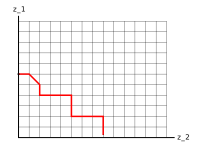
\includegraphics[width=0.8\textwidth]{automata.png}
\end{figure}
\end{frame}

\begin{frame}
\frametitle{Определение маневра}
\begin{my_definition}
  Пусть у нас есть инициализированный автомат с двумя счётчиками.  Конечным манёвром называется
  поведение автомата от момента времени \(t_1\) до \(t_2\),
  если выполняются следующие условия:
  \begin{equation*}
    \begin{cases}
      \forall t (t_1 \leq t < t_2 \Rightarrow q(t) \notin Q_f) \\
      \forall t (t_1 < t < t_2 \Rightarrow (z_1(t) \ne 0 \wedge z_2(t) \ne 0) \\
      \begin{sqcases}
        z_1(t_1) = 0 \wedge z_2(t_1) \ne 0 \wedge z_2(t_2) = 0 \\
        z_2(t_1) = 0 \wedge z_1(t_1) \ne 0 \wedge z_1(t_2) = 0
      \end{sqcases}
    \end{cases}
  \end{equation*}
\end{my_definition}
\end{frame}

\begin{frame}
\frametitle{Определение маневра}
\begin{my_definition}
  Пусть у нас есть инициализированный автомат с двумя счётчиками.  Неполным манёвром называется
  поведение автомата от момента времени \(t_1\) до \(t_2\), если выполняются следующие условия:
  \begin{equation*}
    \begin{cases}
      \forall t (t_1 \leq t < t_2 \Rightarrow q(t) \notin Q_f) \\
      \forall t (t_1 < t \leq t_2 \Rightarrow (z_1(t) \ne 0 \wedge z_2(t) \ne 0)) \\
      \begin{sqcases}
        z_1(t_1) = 0 \wedge z_2(t_1) \ne 0 \\
        z_2(t_1) = 0 \wedge z_1(t_1) \ne 0
      \end{sqcases} \\
      q(t_2) \in Q_f
    \end{cases}
  \end{equation*}
\end{my_definition}
\end{frame}

\begin{frame}
\frametitle{Определение маневра}
\begin{my_definition}
  Пусть у нас есть инициализированный автомат с двумя счётчиками.  Бесконечным манёвром называется
  поведение автомата от момента времени \(t_1\), если выполняются следующие условия:
  \begin{equation*}
    \begin{cases}
      \forall t (t_1 \leq t \Rightarrow q(t) \notin Q_f) \\
      \begin{sqcases}
        z_1(t_1) = 0 \wedge \forall t (t_1 \leq t \Rightarrow z_2(t) \ne 0) \\
        z_2(t_1) = 0 \wedge \forall t (t_1 \leq t \Rightarrow z_1(t) \ne 0)
      \end{sqcases}
    \end{cases}
  \end{equation*}
\end{my_definition}
\end{frame}

\begin{frame}
\frametitle{Функция маневра}

\begin{my_definition}
  \label{def:manoeuvre_function}
  Функция \(f \in \F\) называется функцией маневра, если она имеет один из следующих видов:
  \begin{align*}
    & f(x) =
      \begin{cases}
        C_0, & x = 0 \\
        C_1, & x = 1 \\
        \ldots \\
        C_k, & x = k \\
        \frac{a x + b(x)}{d}, & x > k
      \end{cases}
    \ \ \ \ \ \ \ \ \text{или}
    & f(x) =
      \begin{cases}
        C_0, & x = 0 \\
        C_1, & x = 1 \\
        \ldots \\
        C_k, & x = k \\
        \lambda, & x > k
      \end{cases}
  \end{align*}
\end{my_definition}
\end{frame}

\begin{frame}
\frametitle{Функция с переключателем}

\begin{my_definition}
  Пусть \(g \in \F\).  \(g\) называется переключательной функцией, если
  \(\left|Im(g)\right| < \infty\).
\end{my_definition}

\begin{notation}
  \(\G\) --- множество всех переключательных функции.
\end{notation}

\begin{my_definition}
  Пара \((f, g)\) называется функцией с переключателем, если \({f \in \F, g \in \G}\) и
  \(Def(f) = Def(g)\).
\end{my_definition}

\end{frame}

\begin{frame}
\frametitle{Обобщенная суперпозиция}

\begin{my_definition}
Пусть \((f_0, g_0)\), \((f_1, g_1)\), \((f_2, g_2)\), \ldots,
\((f_n, g_n)\) --- функции с переключателями и
\(Im(g_0) = \{k_1, k_2, \ldots, k_n\}\).
  \(S_n[(f_0, g_0), (f_1, g_1), (f_2, g_2), \ldots (f_n, g_n)]\) -- это пара функций \((f, g)\),
  где \(f\) и \(g\) имеют вид:
  \begin{align*}
    & f(x) =
      \begin{cases}
        f_1(f_0(x)), & g_0(x) = k_1 \\
        f_2(f_0(x)), & g_0(x) = k_2 \\
        \ldots \\
        f_n(f_0(x)), & g_0(x) = k_n
      \end{cases}
    & g(x) =
      \begin{cases}
        g_1(f_0(x)), & g_0(x) = k_1 \\
        g_2(f_0(x)), & g_0(x) = k_2 \\
        \ldots \\
        g_n(f_0(x)), & g_0(x) = k_n
      \end{cases}
  \end{align*}
\end{my_definition}
\end{frame}

\begin{frame}
\frametitle{Специальная рекурсия}

\begin{notation}
Пусть \((f, g) \in \F \times G\) и \(a \in \N_0\).
\begin{align*}
  & \Delta_0(a) = \{x \in \N_0 | g(x) = a\} \\
  & \Delta_{k + 1}(a) = \{x \in \Delta_{k} | g(f^{k + 1}(x)) = a\},\ \text{где}\ k \geq 0 \\
  & X_0(a) = \N_0 \setminus \Delta_0(a) \\
  & X_{k + 1}(a) = \Delta_{k}(a) \setminus \Delta_{k + 1}(a),\ \text{где}\ k \geq 0 \\
  & X_{\infty}(a) = \N_0 \setminus \bigcup_{k \geq 0} X_k(a)
\end{align*}
\end{notation}
\end{frame}

\begin{frame}
\begin{my_definition}
  Пусть \(f_0, g_0 \in \F \times \G\) и \(a \in \N_0\).
  \(R_a[(f_0, g_0)]\) -- это пара функций \((f, g)\),
  где \(f\) и \(g\) имеют вид:
  \begin{align*}
    & f(x) =
      \begin{cases}
        f^{k + 1}_0(x), & x \in X_k(a) \\
        \lambda, & x \in X_{\infty}(a)
      \end{cases} \\
    & g(x) =
      \begin{cases}
        g_0(x), & x \in X_0(a) \\
        g_0(f_0^k(x)), & x \in X_k(a), k \geq 1 \\
        \lambda, & x \in X_{\infty}(a)
      \end{cases}
  \end{align*}
\end{my_definition}
\end{frame}

\begin{frame}
  \frametitle{Пример}
  \begin{align*}
    & f(x) =
      \begin{cases}
        \frac{x}{2}, \text{если}\ x = 2 k \\
        x, \text{если}\ x = 2 k + 1
      \end{cases}
    & g(x) =
      \begin{cases}
        0, \text{если}\ x = 2 k \\
        1, \text{если}\ x = 2 k + 1
      \end{cases}
  \end{align*}
  \begin{align*}
    & \Delta_0(0) = \{x \in \N_0 \mid x = 2 k\}
    & X_0(0) = \{x \in N_0 \mid x = 2 k + 1\} \\
    & \Delta_1(0) = \{x \in \N_0 \mid x = 4 k\}
    & X_1(0) = \{x \in N_0 \mid x = 4 k + 2\} \\
    & \Delta_2(0) = \{x \in \N_0 \mid x = 8 k\}
    & X_2(0) = \{x \in N_0 \mid x = 8 k + 4\} \\
    & \ldots & \ldots \\
    & & X_{\infty}(0) = \{0\}
  \end{align*}
\end{frame}

\begin{frame}
  \frametitle{Пример}
  \begin{align*}
    & (f', g') = R_0[f, g] \\
    & f'(x) =
    \begin{cases}
      \lambda, \text{если}\ x = 0 \\
      x, \text{если}\ x = 2 k + 1 \\
      \frac{x}{2}, \text{если}\ x = 4 k + 2 \\
      \frac{x}{4}, \text{если}\ x = 8 k + 4 \\
      \ldots \\
      \frac{x}{2^n}, \text{если}\ x = 2^{n + 1} k + 2^n \\
      \ldots \\
    \end{cases} \\
    & g'(x) =
      \begin{cases}
        \lambda, \text{если}\ x = 0 \\
        1, \text{если}\ x > 0
      \end{cases}
  \end{align*}
\end{frame}

\begin{frame}
\frametitle{Функция маневра с переключателем}

\begin{my_definition}
  \label{def:periodic}
  Функция \(g \in \G\) называется периодичной, если существуют \(T \in \N\) и \(x_0 \in \N_0\),
  такие что для любого \(x > x_0\) и для любого \(k \in \N_0\) верно \(f(x) = f(x + kT)\).
\end{my_definition}

\begin{my_definition}
  \label{def:manoeuvre_function_switcher}
  Функция с переключателем \((f, g)\) называется функцией маневра с переключателем, если
  выполняются следующие условия:
  \begin{itemize}
    \item \(f\) --- функция маневра
    \item \(g\) --- периодичная функция
    \item шаг маневра \(f\) совпадает c минимальным периодом \(g\)
  \end{itemize}
\end{my_definition}
\end{frame}

\begin{frame}
\frametitle{Обобщенная функция маневра с переключателем}

\begin{my_definition}
  Определим обобщенную функцию маневра с переключателем через индуктивное определение:
  \begin{enumerate}
  \item Любая функция маневра с переключателем это обобщенная функция маневра с переключателем.
  \item Для любых \(n \in \N\) и \(m \in \N_0\) если \((f_0, g_0)\), \((f_1, g_1)\),
    \((f_2, g_2)\), \ldots, \((f_n, g_n)\) являются обобщенными функциями маневра с
    переключателем, то функции
    \((f', g') = S_n[(f_0, g_0), (f_1, g_1), \ldots, (f_n, g_n)]\) и
    \((f'', g'') = R_a[(f_0, g_0)]\) тоже являются обобщенными функциями маневра с
    переключателем.
  \end{enumerate}
\end{my_definition}
\end{frame}

\begin{frame}
\frametitle{Обобщенная функция маневра}
\begin{my_definition}
  Функция \(f\) называется обобщенной функцией маневра, если существует \({g \in \G}\) такая, что
  \((f, g)\) является обобщенной функцией маневра с переключаетелем.
\end{my_definition}

\begin{notation}
  \(\F_2\) --- множество всех обобщенных функций маневра.
\end{notation}
\end{frame}

\begin{frame}
\frametitle{Основной результат}
  \begin{my_theorem}
    Автомат с 2 счётчиками вычисляет функцию \(f\) тогда и только тогда, когда функция \(f\)
    является обобщенной функцией маневра.
  \end{my_theorem}
\end{frame}

\end{document}
